\section{The Decline in Interest Rates and Monetary Policy}

In the selected sample of advanced economies, the results imply heterogeneous effects of the national monetary policy and the U.S. monetary policy. Furthermore, unconventional monetary policy interventions, e.g., quantitative easing programs, yield varying results in different countries. Therefore, I examine the yield movements around the monetary policy decision dates by country.

\subsection{German Bund Yields}

In Figure \ref{fig:german2008} and \ref{fig:german1999}, the cumulative yield change of the 10-year German bunds with respect to both ECB and FOMC announcements is depicted for complete sampled interval and post-crisis period. Figure \ref{fig:german2008} implies that in the post-crisis period, the monetary policy announcements by the ECB appear to be white noise for 10-year German bunds. In contrast, in the pre-crisis period, the yield movements around the ECB monetary policy announcements co-move with the trend. This finding provokes a question of what phenomenon exactly causes this kind of structural break. More specifically, the cumulative yield change and ECB's within-window yield change have almost opposite directions around 2009-2012. Therefore, the effect of the unconventional monetary policy tool of the ECB, namely the Securities Market Programme of 2010-2012, and the effect of the quantitative easing by the Fed are potential causes. Nevertheless, the fragile relationship between the cumulative yield change and ECB's within-window yield and the yield movement is obvious. \\

\begin{figure}[!htbp]
    \centering
    \caption{$\Delta$Yield in 3-days Around the ECB and FOMC Announcements (2008-2024)}   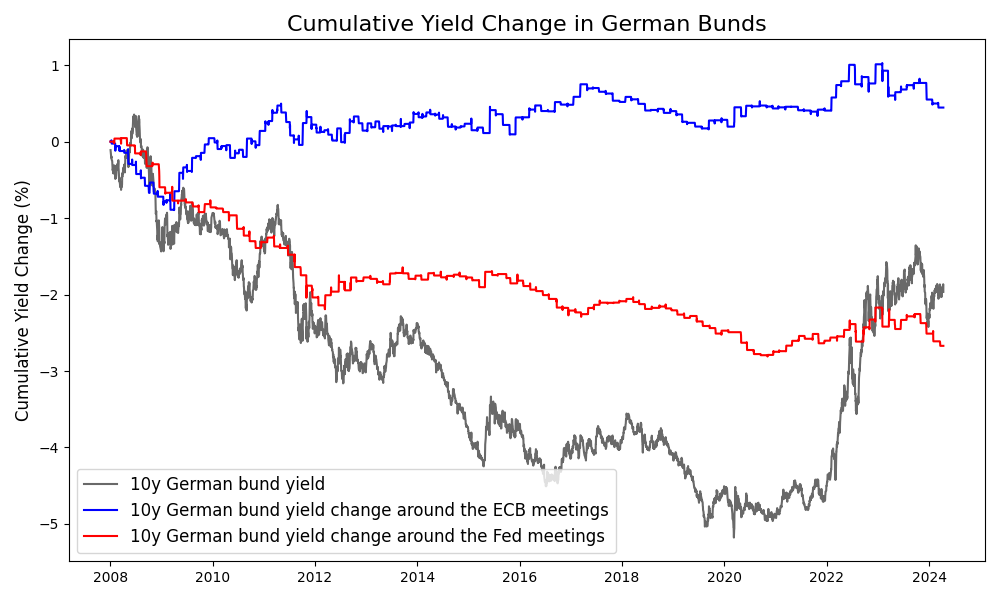
\includegraphics[width=0.9\textwidth]{figures/2008_german_bunds_figure1a.png}
    \label{fig:german2008}
\end{figure}

\begin{figure}[!htbp]
    \centering
     \caption{$\Delta$Yield in 3-days Around the ECB and FOMC Announcements (1999-2024)}   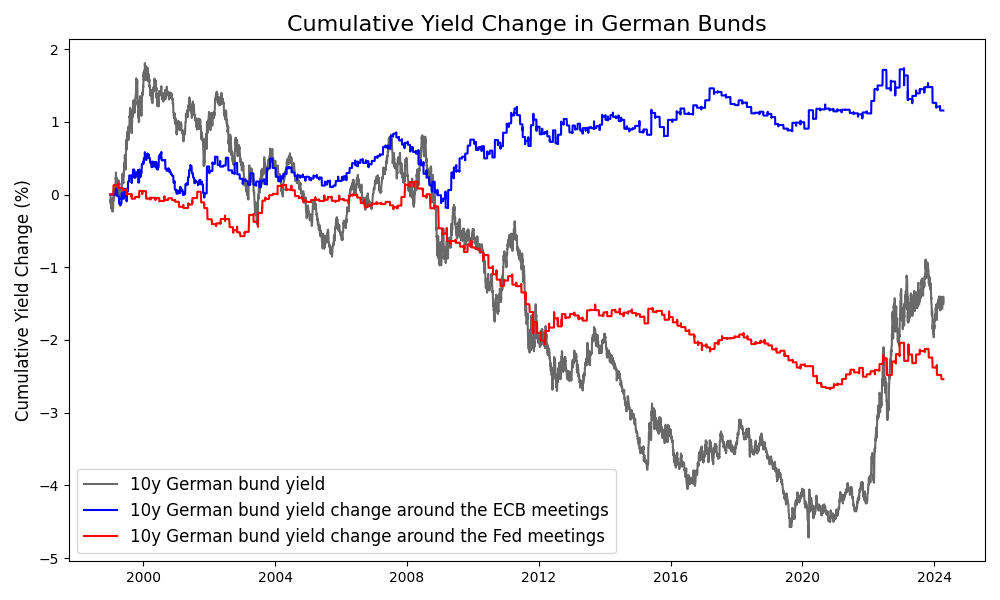
\includegraphics[width=0.9\textwidth]{figures/1999_german_bunds_figure1a.png}

    \label{fig:german1999}
\end{figure}


On the other hand, the yield movements of 10-year German bunds around the FOMC announcements have stronger co-movement with the trend in the whole sample. However, it is important to note that there was a jump around 2012 in this co-movement but the co-movement remained persistent even after that jump. As in the case of the ECB announcements, the question arises as to what caused that jump with potential explanations of the unconventional monetary policy tools. Using a straightforward OLS approach to measure the cross-border monetary policy spillovers from the FOMC announcements to German bunds, I regress the yield change of 10-year German bunds on the yield change of 10-year Treasuries around the 3-day FOMC announcements:

\begin{equation} \notag
    \Delta 10yr_{t-1,t,DE}= \beta_0 + \beta_1\, \Delta 10yr_{t-1,t,US} + \varepsilon_t
\end{equation}
\vspace{-0.25cm}

The results of the spillover regression is depicted in Table \ref{tab:spillreg} and Figure \ref{fig:spillovers}. The estimation to assess the magnitude of cross-border spillovers from 10-year Treasury yields to 10-year German bunds indicates that a one standard deviation change in U.S. Treasury yields corresponds to a 0.44 standard deviation change in German bund yields, highlighting the significant influence of FOMC announcements on German bond markets.


% ======================================

\subsection{UK Gilt Yields}

Figure \ref{fig:uk1999} depicts the yield change of the 10-year government bonds of the United Kingdom, gilts namely, with respect to both BoE and FOMC announcements for both sample intervals, i.e., post-1999 and post-crisis. The simple descriptive evidence suggests a divergence between the German bunds and the UK gilts. That is, neither in pre-crisis nor post-crisis periods, the effect of the BoE's rate announcements became white noise. Instead, regardless of the selected time interval, the yield movements around the BoE and FOMC announcements accounts for the yield movement itself. To see this strong relationship, the yield changes around both meetings are combined in Figure \ref{fig:uk1999both}. \\

Moreover, in contrast to other countries in the sample, the fact that the decline in bond yields could be explained by the decline in the 3-day windows around the BoE's decisions may indicate that the BoE, unlike other central banks in the sample, enjoys relatively stronger monetary authority and a certain degree of autonomy in the face of the Global Financial Cycle. While the UK's divergence from other countries requires a more in-depth macroeconomic analysis, the fact that the 3-day windows around the BoE and FOMC announcements explain the decline in long-term bond yields confirms that, contrary to conventional thinking, monetary policy is likely to explain the decline in long-term interest rates. Lastly, the result of regressions yield change of 10-year UK gilts on the yield change of 10-year Treasuries around the 3-day FOMC windows indicate that for one standard deviation decline in the 10-year Treasuries is associated with 0.49 standard deviation decline in the 10-year UK gilts, confirming the cross-border monetary spillovers.

\begin{figure}[!htbp]
    \centering
    \caption{$\Delta$Yield in 3-days Around the BoE and FOMC Announcements (1999-2024)}    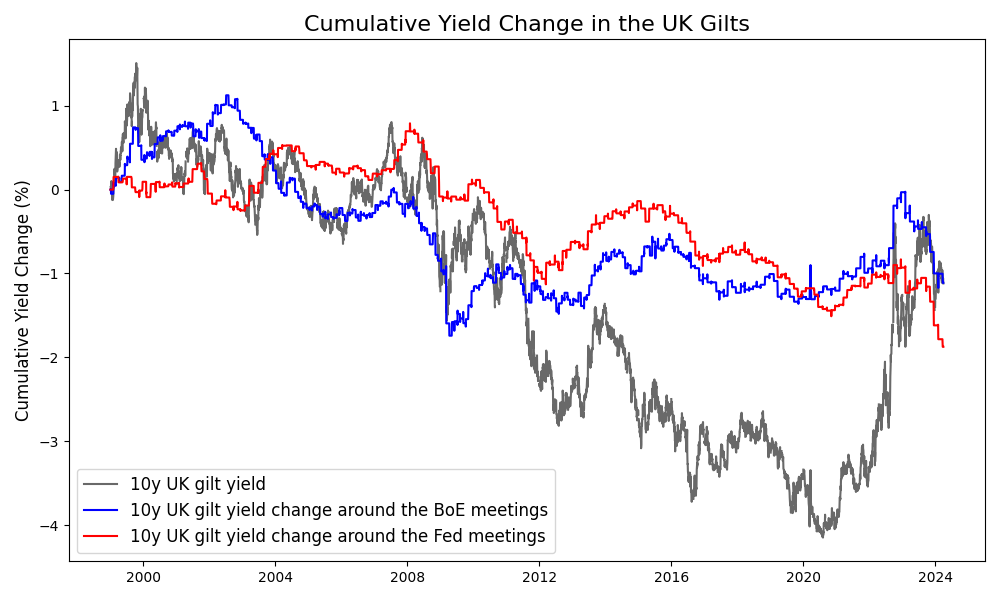
\includegraphics[width=0.9\textwidth]{figures/1999_uk_gilts_figure1a.png}
    \label{fig:uk1999}
\end{figure}
\vspace{0.2cm}

\begin{figure}[!htbp]
    \centering
    \caption{$\Delta$Yield in 3-days Around the Both CBs' Announcements (1999-2024)}    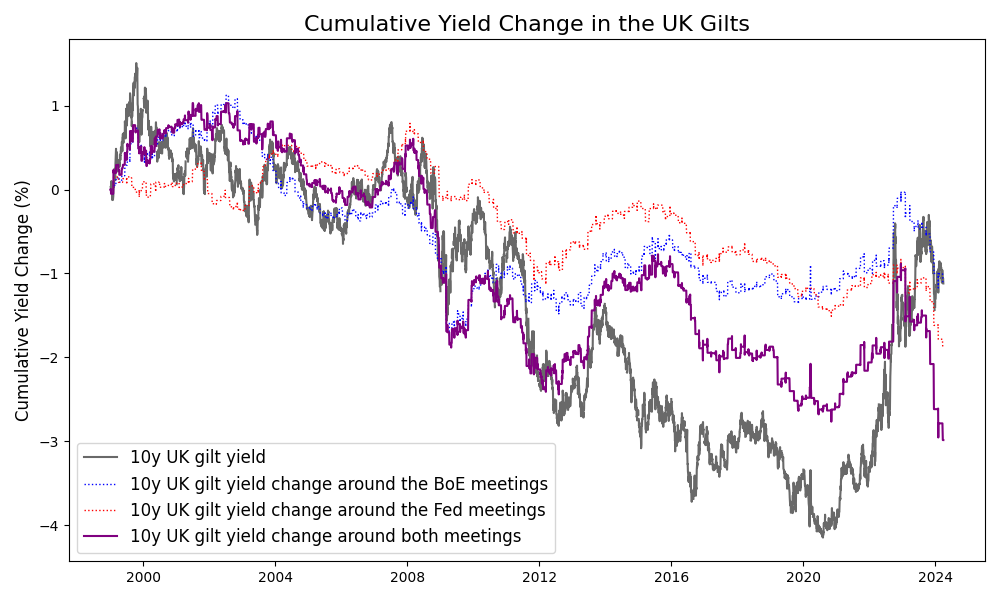
\includegraphics[width=0.9\textwidth]{figures/1999_uk_gilts_figure1a_combined.png}

    \label{fig:uk1999both}
\end{figure}


% ======================================

\subsection{Japanese Government Bond (JGB) Yields}

Figure \ref{fig:boj1997} illustrate the yield movements of 10-year Japanese Government Bonds (JGBs) including 3-day time window change with respect to the FOMC and BoJ announcements, for both post-1997 and post-crisis intervals. In line with the findings in the Germany case, it is evident that there was a striking structural break around the Global Financial Crisis. A more thorough analysis shows that the break occurred approximately between 2006 and 2008. From 1997 until the Global Financial Crisis, the 3-day yield windows built around the BoJ announcements captured the change in bond yields to a large degree and in tandem with the trend, whereas in the post-crisis period, the change in bond yields became insensitive to BoJ announcements. On the other hand, as shown in Figure \ref{fig:boj1997}, the 3-day windows around the FOMC announcements in the post-crisis period largely account for the change in bond yields. To observe this pattern more precisely, see Figure \ref{fig:boj97mix}, which depicts the time windows around the BoJ announcements in the pre-crisis period and the time windows around the FOMC in the post-crisis period. Additionally, the coefficient for the cross-border monetary spillover regression, presented in Table \ref{tab:spillreg} and Figure \ref{fig:spillovers}, illustrates that at the 0.05 significance level, the decline in the U.S. Treasuries spills over the Japanese long-term government bonds. In terms of economic significance, for one standard deviation decline in the U.S. Treasuries lead 0.1 standard deviation decline in Japanese bonds.\\

\begin{figure}[!htbp]
    \centering
     \caption{$\Delta$Yield in 3-days Around the BoJ and FOMC Announcements (1997-2024)}   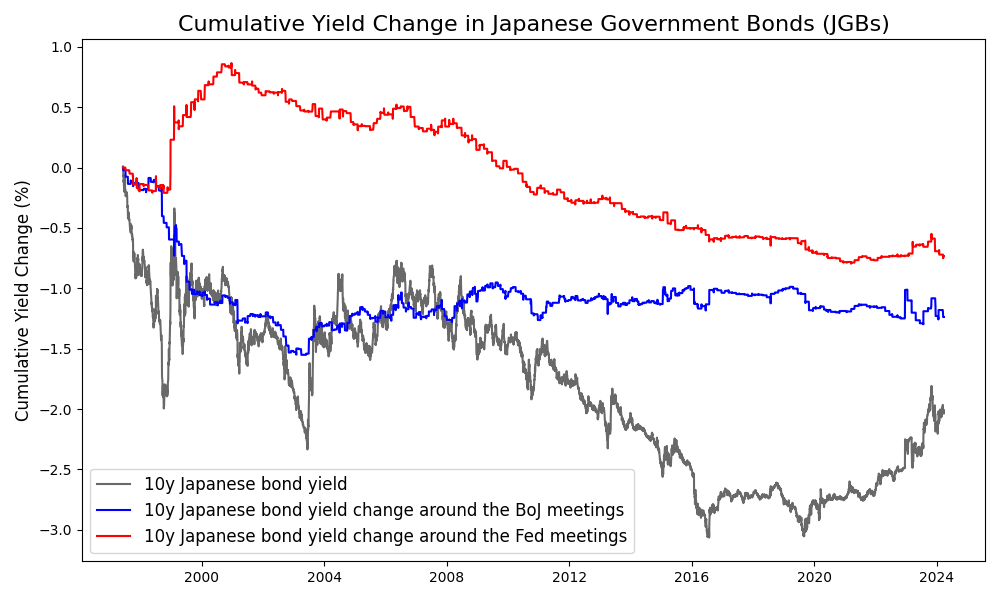
\includegraphics[width=0.9\textwidth]{figures/1997_japanese_bonds_figure1a.png}

    \label{fig:boj1997}
\end{figure}

While on the one hand, the patterns of this change brought about by the Global Financial Crisis are evident and raise the question of the amplification of the Global Financial Cycle, on the other hand, questions remain about the impact of unconventional monetary policy tools on this outcome. As in the case of Germany, the ECB's Securities Market Program of 2010-2012 is being discussed, whether the Japanese QE program, which ended in 2006, had an impact on this structural break remains a noteworthy research agenda.



\begin{figure}[!htbp]
    \centering
    \caption{$\Delta$Yield Around the Altered BoJ-FOMC Announcements (1997-2024)} 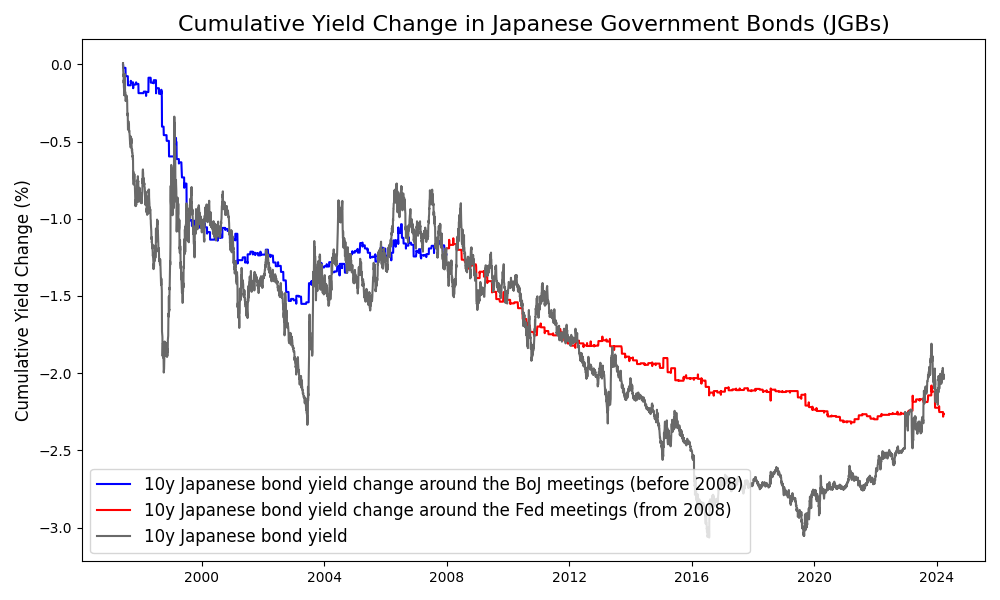
\includegraphics[width=0.9\textwidth]{figures/1997_japanese_mixed.png}

    \label{fig:boj97mix}
\end{figure}

% ======================================

\subsection{Canadian Bond Yields}

Due to spatial proximity and entangled economic and financial relationships, Canada has a particular status in the sample. Employing a global VAR model, \citet{beaton2011financial} emphasizes the significance of financial variables in transmission of shocks from the U.S. to Canada, including both disturbances to real economic activity and to financial conditions. Financial linkage, combined with robust trade relations and geographical proximity, would be likely spillovers from the U.S. monetary policy decisions to Canadian economy and to Canadian bond yields in particular. Indeed, in both the post-1999 and post-crisis sample, depicted in Figures \ref{fig:canada2008} and \ref{fig:boc1999}, it is obvious that Canadian bond yield movements in the 3-day time windows of the FOMC announcements account for the overall trend in Canadian bond yields. As deep-rooted economic entanglements might suggest, there is no evident structural break per se around the Global Financial Crisis that intensified the evidence for the Global Financial Cycle.

\begin{figure}[!htbp]
    \centering
    \caption{$\Delta$Yield in 3-days Around the BoC and FOMC Announcements (2008-2024)}
    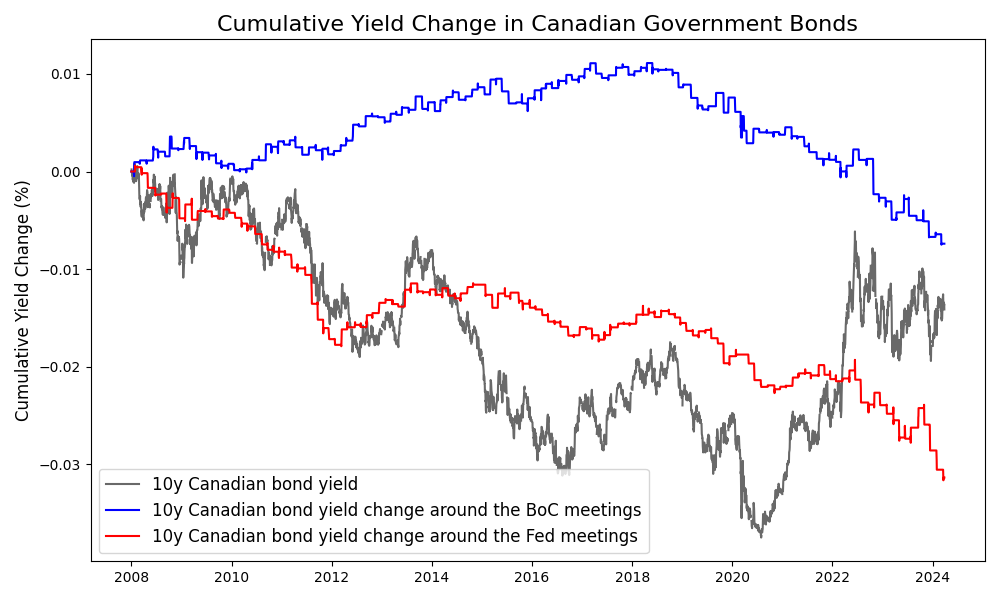
\includegraphics[width=\textwidth]{figures/2008_canadian_bond_figure1a.png}
    \label{fig:canada2008}
\end{figure}


\begin{figure}[!htbp]
    \centering
    \caption{$\Delta$Yield in 3-days Around the BoC and FOMC Announcements (1999-2024)}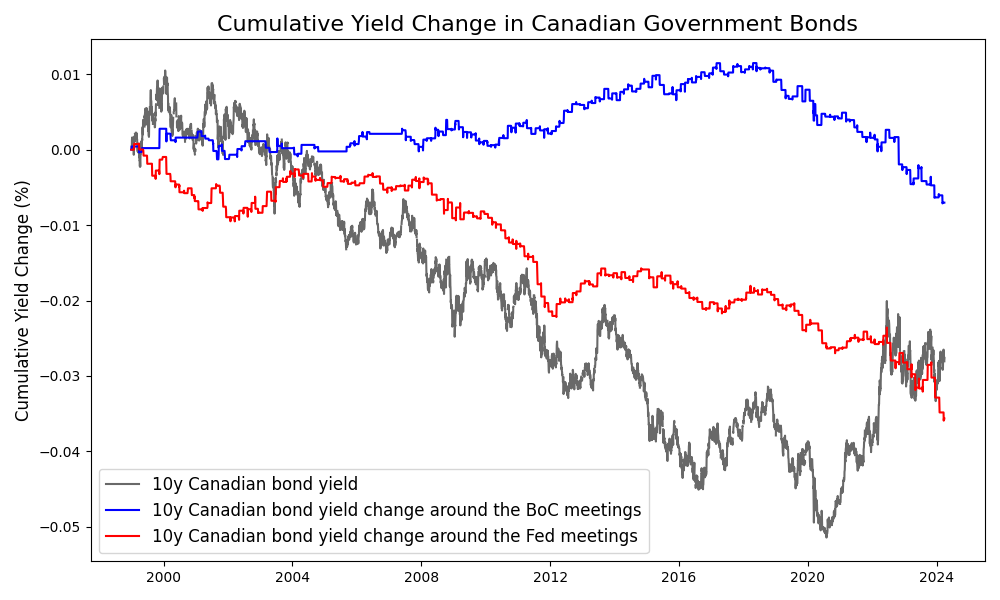
\includegraphics[width=0.9\textwidth]{figures/1999_canadian_bond_figure1a.png}

    \label{fig:boc1999}
\end{figure}

Using the cross-border spillover regressions as in the previous cases, the results are particularly striking. Illustrated in Table \ref{tab:spillreg}, 100 basis points decline in the U.S. Treasuries is associated with 59 basis points decline in the long-term Canadian bonds around the 3-day FOMC announcement windows, and this result is statistically significant at the 0.01 level. Standardizing for the results, for one s.d. change in U.S. Treasuries is associated with 0.81 change in Canadian bond yields.

\subsection{Swiss Confederation Bond Yields}

Figure \ref{fig:snb2008} and \ref{fig:snb2000} accurately indicate that neither the 3-day windows around the FOMC meetings nor those around the Swiss National Bank meetings have any explanatory power of declining long-term yields. Furthermore, there exist no structural breaks attributable to the Global Financial Crisis. This descriptive result is partly supported by the cross-border spillover regression. In the Column 5 of Table \ref{tab:spillreg}, for 100 basis points decline in the U.S. Treasuries, the yield change in the 10-year Swiss Confederation Bonds is 10.5 basis points. Given that these results differ significantly from those of other countries in the sample, further investigation is warranted. \\

There are significant macro-financial differences between Switzerland and the rest of the sample. First, the statistics and \citet{cwik2024fx} suggest that the Swiss National Bank conducts sizeable currency intervention in order to influence inflation or to protect the ``safe haven'' status of the Swiss Franc. Further, \citet{bacchetta2022understanding} states that the exchange rate affects the real interest rates in Switzerland, through the convenience yield, mediated by a valuation effect.


\subsection{Australian Government Bond Yields}

Figures \ref{fig:rba2008} and \ref{fig:rba1997} exhibit a overview compared to the previous figures. This is mainly because neither the Fed's nor the RBA's 3-day monetary policy decision windows seem to have much impact on 10-year bond yield changes. Indeed, if observing the trend, the bond yield movement in the RBA decision windows is in the opposite direction to the trend in bond yields. On the other hand, even if the Fed's influence on bond movements is less than in other cases such as Canada or Germany, there is a noticeable co-movement, especially in certain sub-time periods. Nevertheless, this weak and ineffectual co-movement can only account for a too little portion of the variation. For the spillovers around the 3-day FOMC announcement windows, the explained variation of this regression is restricted to 0.009, while the standardized coefficient suggests that for a one standard deviation decline in the U.S. Treasuries, the decline in the Australian Government Bonds is only 0.096 standard deviation. 

\begin{figure}[!htbp]
    \centering
     \caption{$\Delta$Yield in 3-days Around the SNB and FOMC Announcements (2008-2024)}   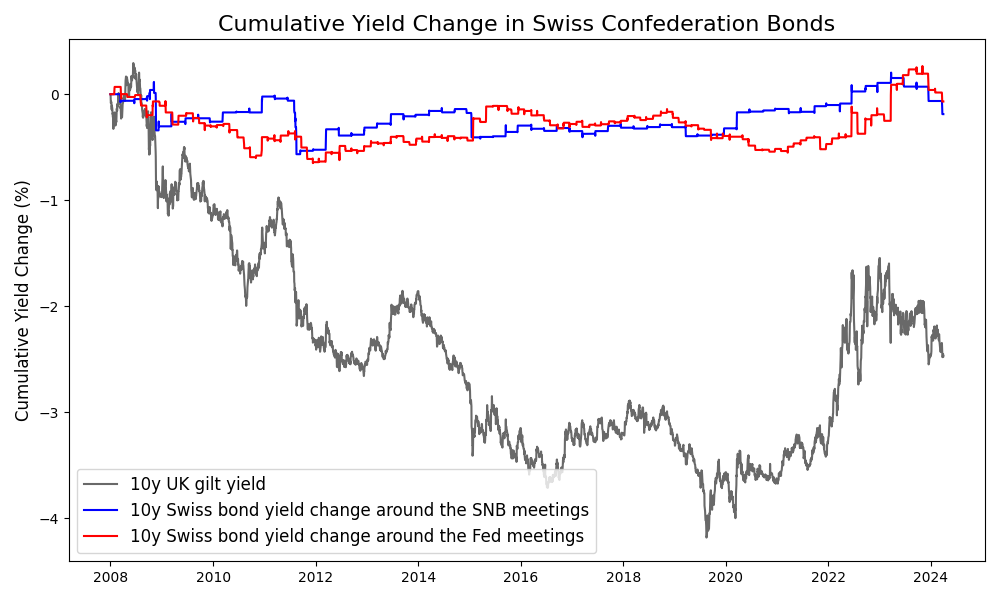
\includegraphics[width=0.9\textwidth]{figures/2008_swiss_bonds_figure1a.png}

    \label{fig:snb2008}
\end{figure}

\begin{figure}[!htbp]
    \centering
    \caption{$\Delta$Yield in 3-days Around the SNB and FOMC Announcements (2000-2024)}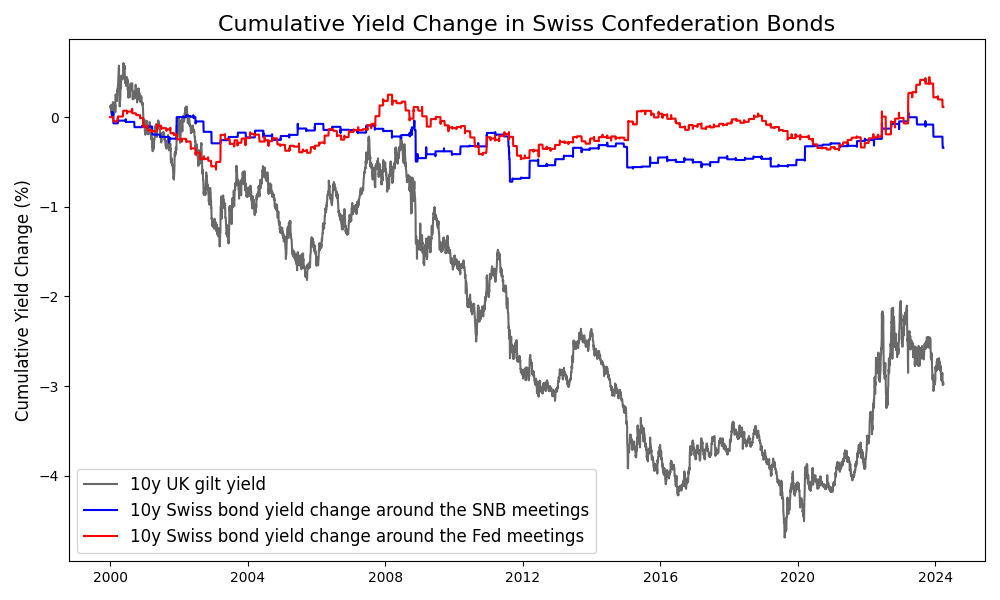
\includegraphics[width=0.9\textwidth]{figures/2000_swiss_bonds_figure1a.png}

    \label{fig:snb2000}
\end{figure}

\FloatBarrier

% ======================================


\begin{figure}[!htbp]
    \centering
    \caption{$\Delta$Yield in 3-days Around the RBA and FOMC Announcements (2008-2024)}    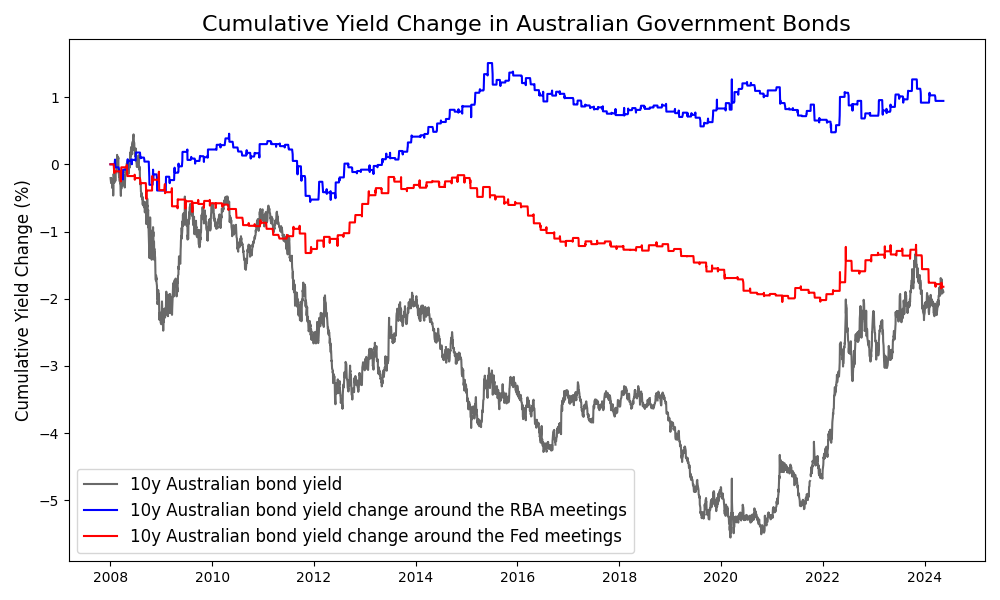
\includegraphics[width=0.9\textwidth]{figures/2008_australian_bonds_figure1a.png}

    \label{fig:rba2008}
\end{figure}

\begin{figure}[!htbp]
    \centering
    \caption{$\Delta$Yield in 3-days Around the RBA and FOMC Announcements (1997-2024)}    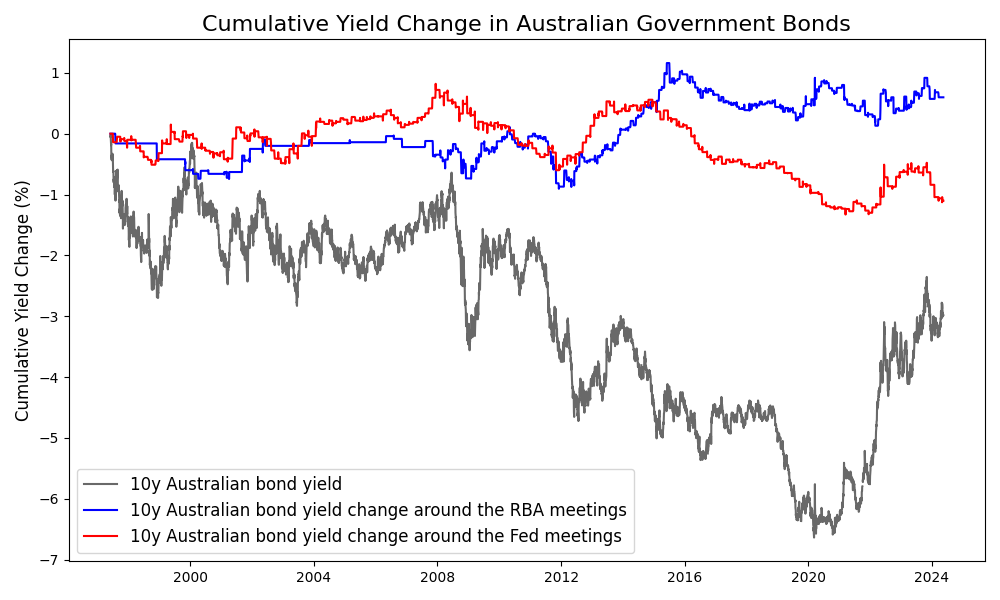
\includegraphics[width=0.9\textwidth]{figures/1997_australian_bonds_figure1a.png}

    \label{fig:rba1997}
\end{figure}

\newpage
% ======================================

\begin{figure}[!htbp]
    \caption{Spillovers from 10yr Treasury to Government Bonds Around FOMC Meetings}
    \centering
    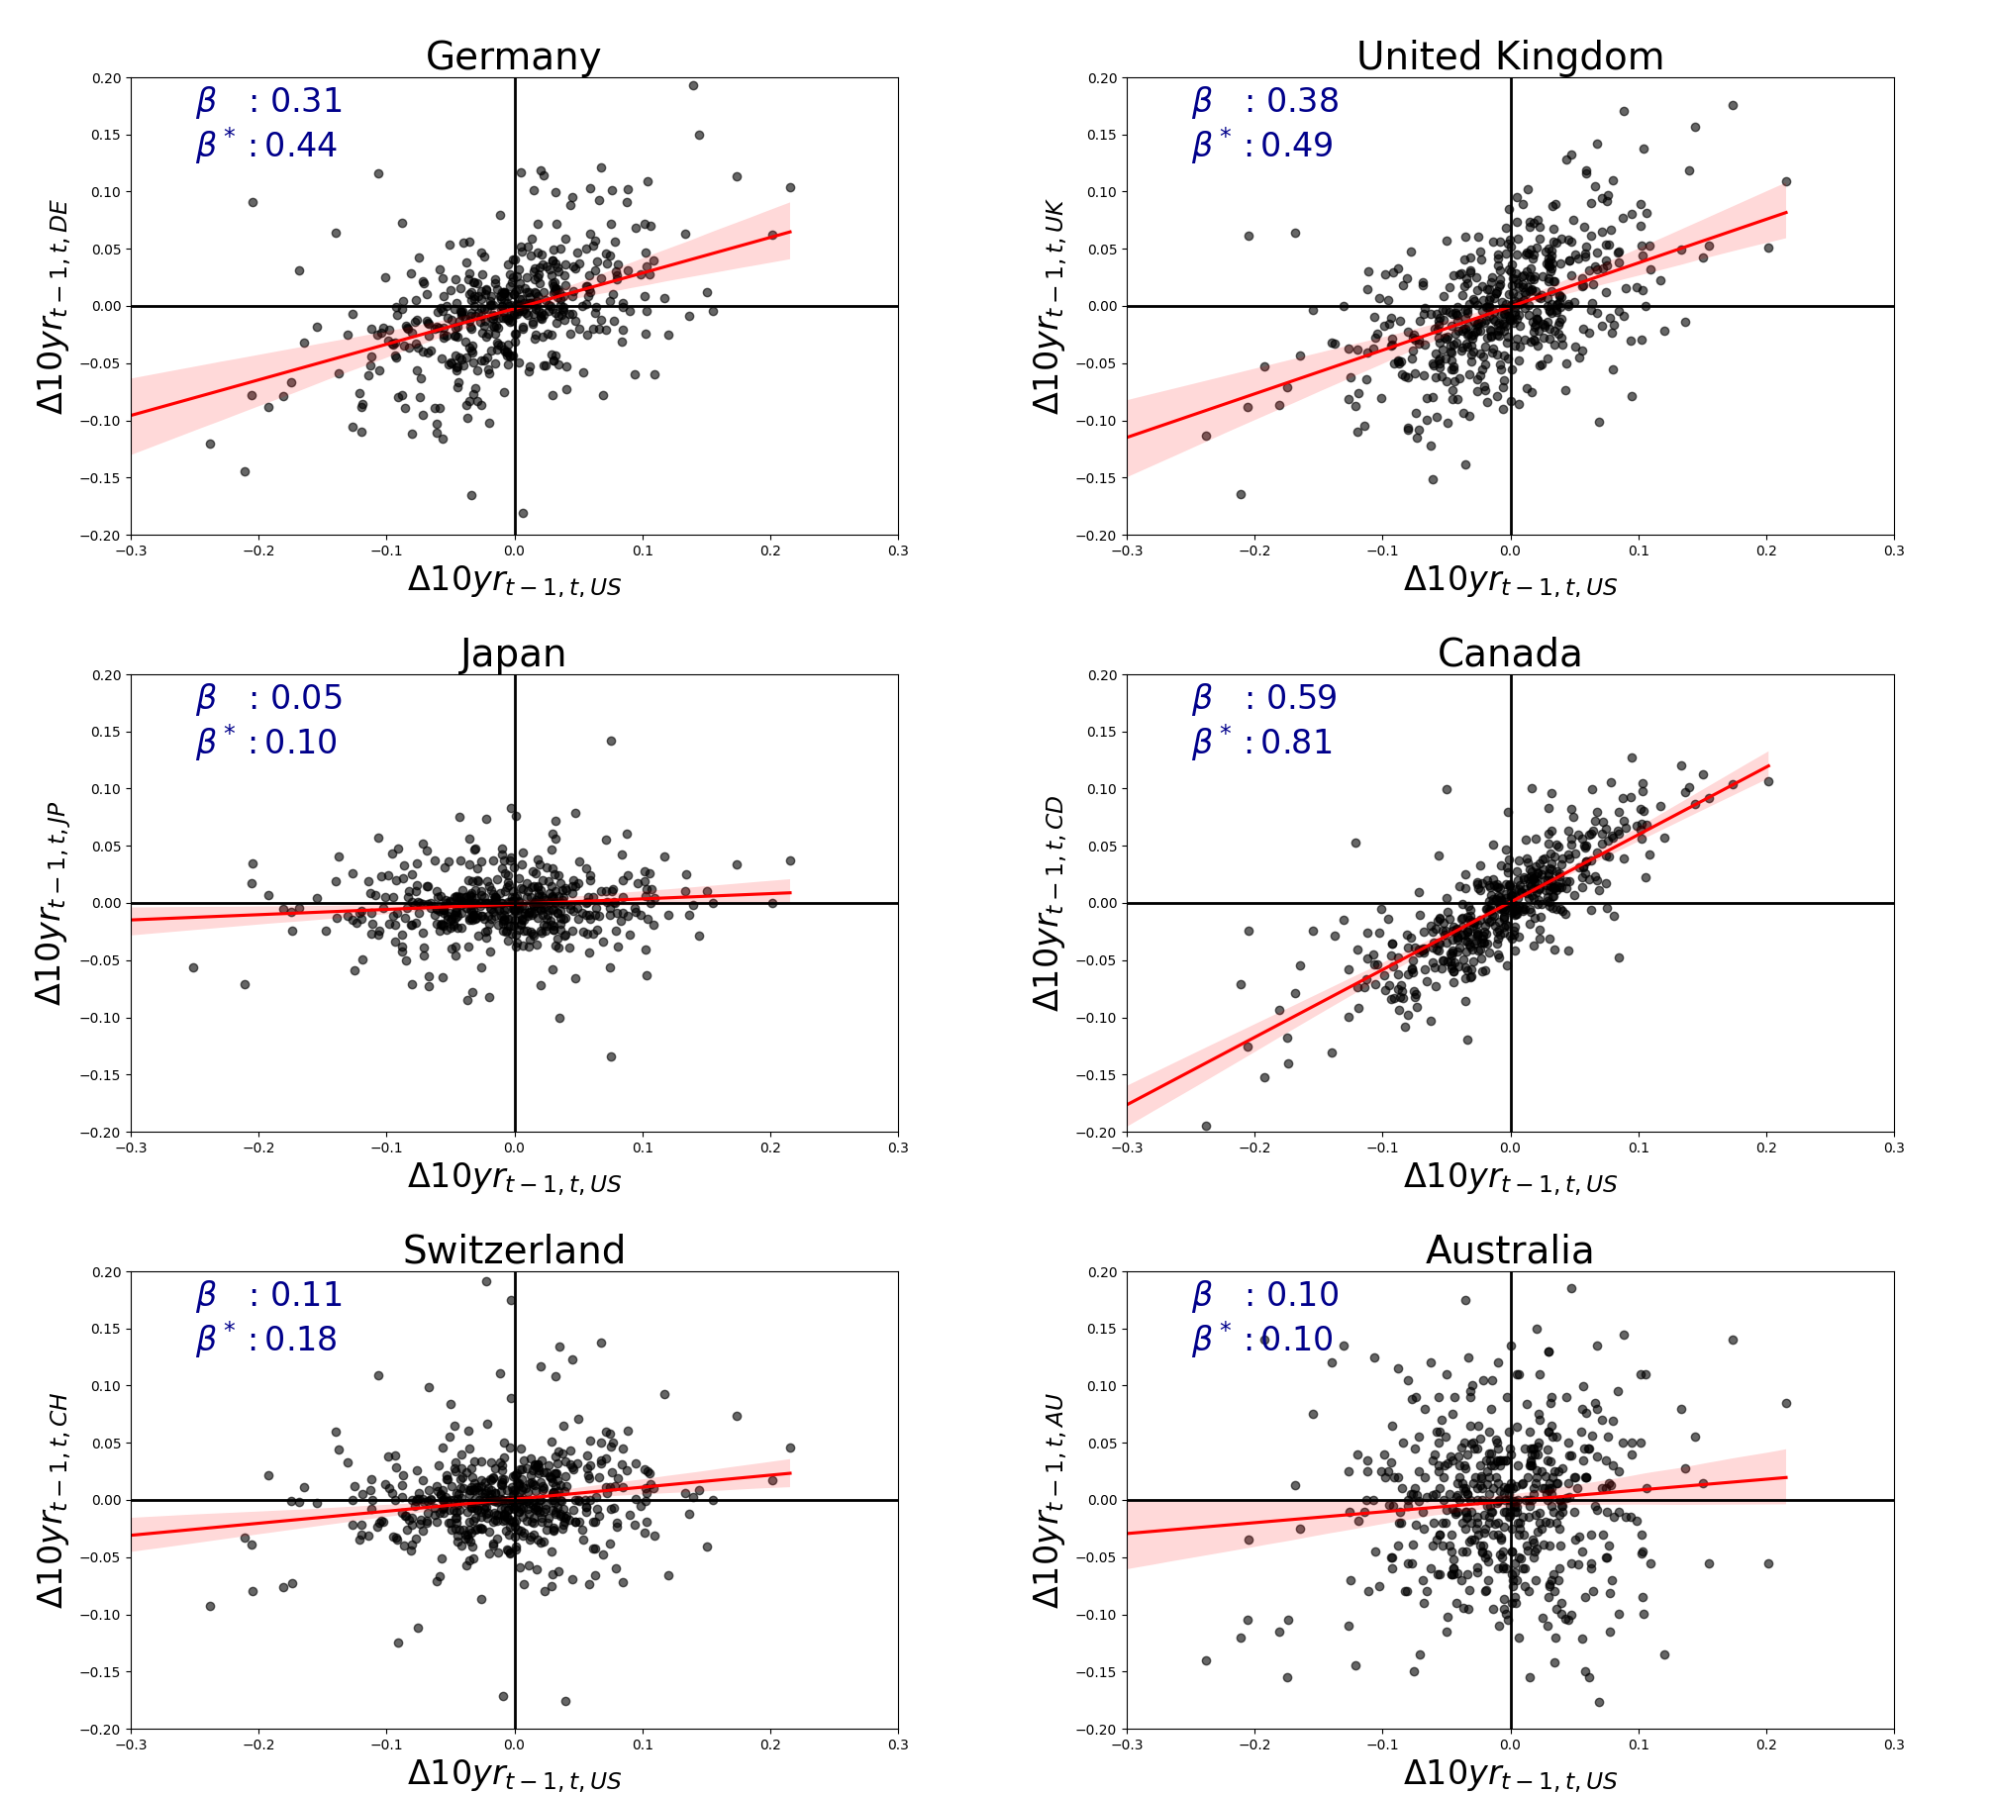
\includegraphics[width=\textwidth]{figures/bondspillovers.png}
    \label{fig:spillovers}
\end{figure}

\begin{table}[!htbp]
\caption{Spillovers from 10yr Treasury to Government Bonds Around FOMC Meetings}
\centering
\begin{tabular}{lcccccc}
\toprule
& \multicolumn{6}{c}{$\Delta$10yr_{Home}} \\
\cmidrule(lr){2-7}
& \multicolumn{1}{c}{Germany} & \multicolumn{1}{c}{UK} & \multicolumn{1}{c}{Japan} & \multicolumn{1}{c}{Canada} & \multicolumn{1}{c}{Switzerland} & \multicolumn{1}{c}{Australia} \\
\midrule
$\Delta$10yr_{US} & 0.311$^{***}$ & 0.382$^{***}$ & 0.046$^{**}$ & 0.591$^{***}$ & 0.105$^{***}$ & 0.095$^{**}$ \\
& (0.029) & (0.030) & (0.021) & (0.019) & (0.024) & (0.043) \\
Std. $\Delta$10yr_{US} & 0.44 & 0.49 & 0.1 & 0.813 & 0.182 & 0.095 \\
\midrule
Observations & 477 & 523 & 494 & 482 & 543 & 535 \\
$R^2$ & 0.193 & 0.241 & 0.010 & 0.661 & 0.033 & 0.009 \\
\bottomrule
\end{tabular}
\label{tab:spillreg}
\end{table}
